%!TEX root = main.tex
\color{black}

\section{Data Collection, Analysis and Labeling}\label{sec:data}

Malware classification is non-deterministic task, as several nuances make vendors disagree on what they classify as malware. Not only subtleties related to programs such as \emph{adware} or \emph{remote management consoles}, for which one can find arguments to classify them in either class, but also because some vendors are more accurate than others when classifying malware.

In order to be able to study how \emph{temporal consistency} and \emph{ground truth} influences a model trained to detect malicious and non-malicious applications, we gathered a large dataset of publicly available samples that includes both \emph{malware} and \emph{goodware} with no a priori labeling.

In this section we will provide an overview of the collected data, in particular its sources, followed by an analysis on these samples, and a discussion on the cross-checking mechanisms we used to perform the labeling. In the end of this section we will provide 3 metrics for analysis that differ in the confidence one can provide on the samples' labeling.

\subsection{Data Sources}\label{sub_sec:data_collection}

To study how \emph{temporal consistency} and \emph{ground truth} influences a model trained to detect malicious and non-malicious applications, we started by gathering a dataset of malware and goodware.
This dataset was obtained from \emph{Malwr}~\cite{tool:malwr}, an online service that runs static and dynamic analysis on user submitted files using \emph{Cuckoo Sandbox}~\cite{tool:cuckoo}.
Although Malwr accepts any kind of file, we are interested solely in \gls{pe} files, not only because Windows' systems are relevant targets of malicious applications, but also due to the fact that our initial approach will focus on static information obtained from these \gls{pe} files.

Malwr service provides the analysis of the submitted files as well as the MD5 of such files, but no labeling as whether a sample corresponds to a malicious or non-malicious application.
To perform this labeling we use the anti-virus' signatures given by \emph{VirusTotal}~\cite{tool:virustotal} at the time of analysis (incorporated in Malwr's reports), as a means of labeling the gathered reports.
VirusTotal is an online service where one can submit a suspicious file and in return obtain a list with the analysis performed by a significant number of vendors on whether the sample is clean or not. 

However, and as mentioned before, these classifications are not unanimous, and we still need to assign a labeling to each sample.
For this reason, we enrich our knowledge regarding samples' ground truth by aggregating metadata from \emph{\gls{nsrl}}~\cite{tool:nsrl} and \emph{VirusShare.com}~\cite{tool:virusshare}, specifically the samples' MD5. 
NSRL contains a collection of digital signatures of known, traceable software applications, whereas VirusShare.com is a repository of malware samples, so a sample belonging to the \gls{nsrl} set gives us a higher confidence that it is indeed goodware, whereas one belonging to VirusShare.com set gives us a higher confidence that it is malware. 

In summary, we collected reports from the \gls{pe} samples available in Malwr, and complemented it with metadata from \gls{nsrl} and VirusShare. The following subsection quantifies our \textit{corpus}, providing a better understanding of the available samples.


\subsection{Data Analysis}\label{sub_sec:data_analysis}
We collected our data from Malwr between April 16th, 2013 and October 10th, 2016.
Our data can be divided in three sets:
\begin{enumerate*}[label={\alph*)},font={\color{red!80!black}\bfseries}]
	\item a set $\RR$ of raw reports, containing 388,702 \gls{pe} samples; 
	\item a set $\CC\subseteq\RR$ of 284,880 classified reports by 38 vendors ($\mathcal{V}$) that is obtained by restricting the original set $\RR$ (that includes 97 vendors) to those reports whose vendors are present in at least 95\% of the classified samples.
\end{enumerate*}
% Our working dataset $\DD=\CC\subseteq\RR$, is of size 280,391 (72.17\% of $\RR$).

With regards to duplicated submissions, there are 27,798 samples submitted more than once, for a total of 74,916 duplicated submissions $\Cdups$ averaging 2.7 submissions per duplicate.
Understanding how vendors change their signatures on samples is crucial, as we use it to label the dataset. With this in mind, and inspired by Miller et al.~\cite{miller:rev_int}, we start our analysis by studying the differences between the number of positive (\ie\ a sample of malware) and negative (\ie\ a sample that is not malware) classifications over the last and first submission of the same sample.


%%%%%%%%%%%%%%%%%%%%%%%%%%%%%%%%%%%%%%%%%%%%%%%
% From Data Analysis 2 notebook
For each duplicated sample in $\Cdups$ we counted the number of positive classifications on the first and last submissions, $\Pf$ and $\Pl$ respectively.
If $\Pf > \Pl$ then we are looking at a possible \emph{false positive (FP)}, as the number of vendors classifying the sample as malware decreased. Conversely,  if $\Pl > \Pf$ we are looking at a potential \emph{false negative (FN)}. For the case $\Pf=\Pl$ we conclude that vendors are confident regarding their classification for the sample.

Figure \ref{fig:distribution_changes} shows the frequency of $\Pl-\Pf$ for each duplicated sample. We first note that 44.32\% of duplicated samples change in classification, among which 38.72\% increase its classification, whereas only 5.61\% decrease.
Such discrepancy between positive and negative changes suggest a preference for false negatives over false positives, as also noted by Miller et al.~\cite{miller:rev_int}.

\begin{figure*}[]
% 	\centering
	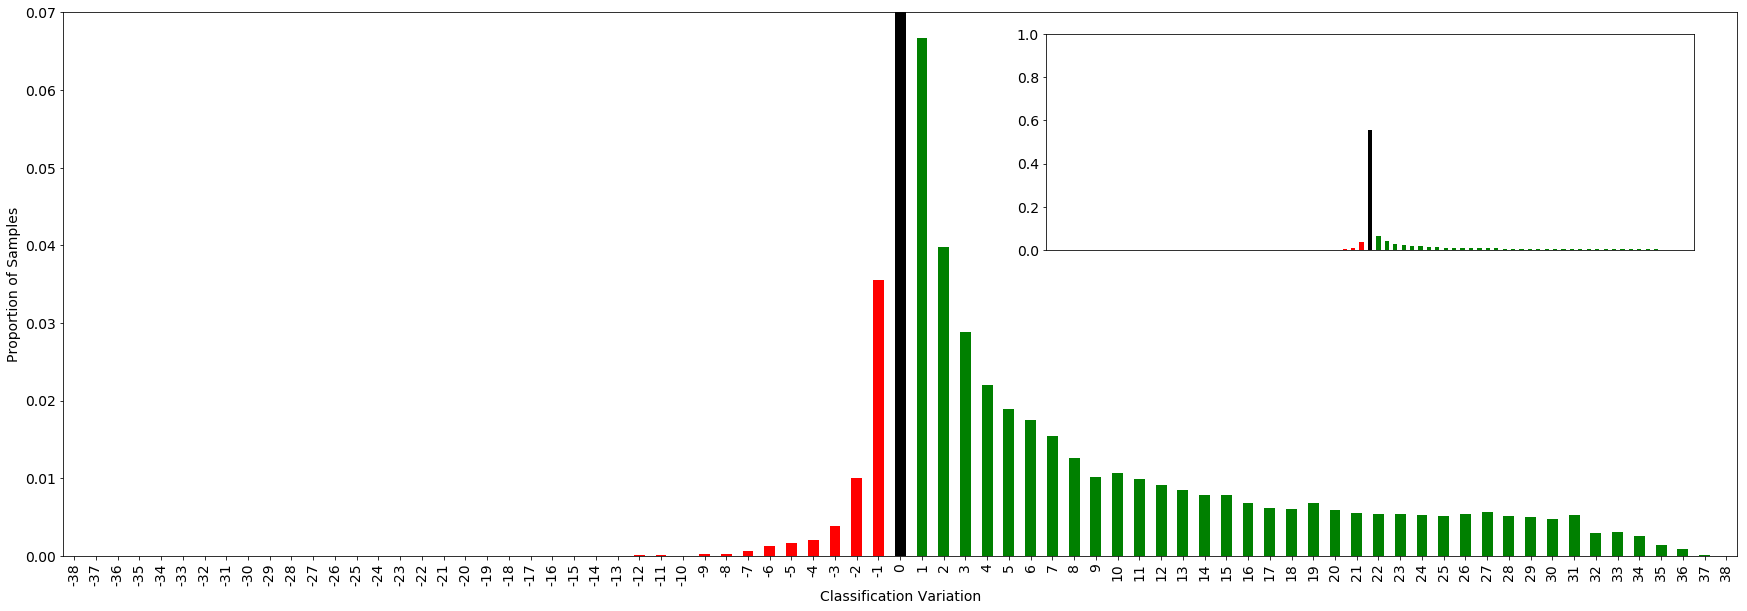
\includegraphics[width=\textwidth]{dups_frequency}
	\caption{Distribution of samples in terms of the changes in the number of positive classifications between last and first submissions, ($\Pl-\Pf$).}
	\label{fig:distribution_changes}
\end{figure*}

\medskip

Another interesting analysis on our dataset is understanding the vendors \emph{\gls{dr}} (or True Positive Rate), and \emph{\gls{fpr}}. 
Although these formulas are trivially defined respectively as
\begin{eqnarray}
\dr&=&\frac\tp{\#malware}=\frac\tp{\tp+\fn} \\ 
\fpr&=&\frac\fp{\#goodware}=\frac\fp{\tn+\fp}
\end{eqnarray}
%{\#goodware}, 
we lack ground truth for what is ${\#malware}$ and $\#goodware$.
To solve this, we propose relative metrics to compute what is positive ($\#malware$) and negative ($\#goodware$).


Our first approach is to take advantage of duplicated submissions to define an accuracy metric, $\Madups$.
As we have previously shown, 44.32\% of duplicated samples change in classification, which can be translated into vendors acknowledging their own errors.

With that in mind, for each vendor $v\in\VV$, we define a duplicated sample for $v$ (according to $\Madups$) as:
\begin{itemize}%[\IEEEsetlabelwidth{Z}]
	\item $\tp_v$, \emph{true positive for $v$}, if $v$ classified it positively in both the first and last submissions;
	\item $\tn_v$, \emph{true negative for $v$}, if $v$ classified it negatively in both the first and last submissions;
	\item $\fp_v$, \emph{false positive for $v$}, if $v$ classified it positively in the first submission and negatively in the last submission;
	\item $\fn_v$, \emph{false negative for $v$}, if $v$ classified it negatively in the first submission and positively in the last submission.
\end{itemize}

Figure~\ref{fig:dr_fpr_own} plots each vendors' $\dr_v$ vs.\ $\fpr_v$. We note that vendors do acknowledge their classification errors, as we see a detection rate from 56.82\% to 85.29\%, with a false positive rate ranging from 0.03\% to 6.91\%. 
Had they kept their original classification, one would have that $\Pl-\Pf = 0$ for every duplicate and consequently $\dr_v = 1$ and $\fpr_v = 0$. 
Notice that by keeping the original classification all clean samples remain clean, hence $\fn_v=0$, and all malicious samples remain malicious, hence $\fp=0$.

\begin{figure}[!h]
	\centering
	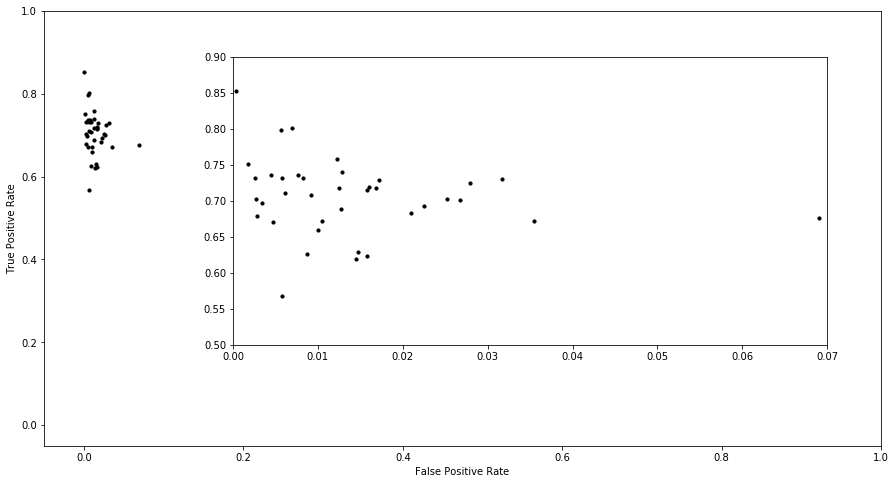
\includegraphics[width=\columnwidth]{dr_fpr_own}
	\caption{$\tpr_v$ vs. $\fpr_v$ according to $\Madups$.}
	\label{fig:dr_fpr_own}
\end{figure}

\medskip

For our second approach regarding vendors' accuracy, we take into account our observations from Figure~\ref{fig:distribution_changes} and our dataset $\CC$ to define another metric $\Mad$.

Intuitively a sample is classified as goodware according to this metric, \ie\ negative, if every vendor $v\in\mathcal{V}$ classifies it as clean.
To understand if our intuition is sound, we plot Figure~\ref{fig:distribution_clean}, a subset of Figure~\ref{fig:distribution_changes}, showing the frequency $\Pl-\Pf$ for samples that were classified as clean in their first submission, \ie, samples with $\Pf=0$. 
These account for 4,902 samples, 3,741 (76.32\%) of which do not increase in classification.

\begin{figure}[!h]
	\centering
	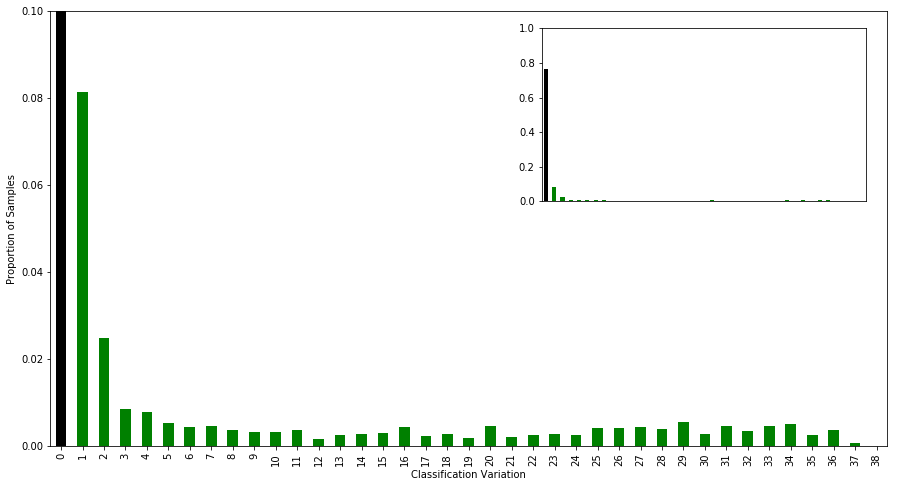
\includegraphics[width=\columnwidth]{distribution_clean}
	\caption{Distribution of samples that started as goodware and changed in the number of positive classifications between the last and first submission, \ie, $\Pl-\Pf$ for samples with $\Pf=0$}
	\label{fig:distribution_clean}
\end{figure}

To arrive at a positive (\ie\ malware) sample definition, we relate Figure \ref{fig:distribution_clean} with Figure \ref{fig:distribution_changes}.
Specifically we want to find a minimum threshold of positive classifications to define a sample as malware.
We chose five as the threshold, observing that percentage of samples that decrease in 5 or more positive classifications is 0.46\%, meaning it is an upper bound for samples that decrease from 5 or more to zero classifications. 

With the previous definitions, we can define a vendors' $v$ classification (according to $\Mad$) as:

\begin{itemize}%[\IEEEsetlabelwidth{Z}]
	\item $\tp_v$, \emph{true positive for $v$}, if $v$ and at least 5 other vendors in $\mathcal{V}$ classify it positively;
	\item $\tn_v$, \emph{true negative for $v$}, if $v$ and all other vendors in $\mathcal{V}$ classify it negatively;
	\item $\fp_v$, \emph{false positive for $v$}, if $v$ is the only vendor in $\mathcal{V}$ classifying it positively;
	\item $\fn_v$, \emph{false negative for $v$}, if $v$ classifies it negatively and at least 5 other vendors in $\mathcal{V}$ classify it positively.
\end{itemize}

Figure \ref{fig:dr_fpr_d} plots each vendors' $\dr_v$ vs. $\fpr_v$ according to~$\Mad$.
Using this metric we note that vendors' detection rate is more scattered than under $\Madups$, ranging from 20.17\% to 83.50\%, whereas false positive rate is similar, ranging from 0.01\% to 5.77\%.

\begin{figure}[!h]
	\centering
	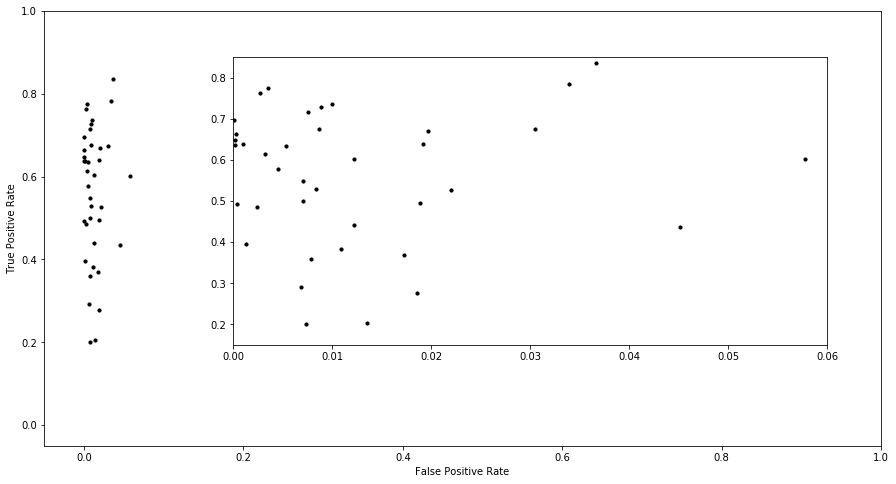
\includegraphics[width=\columnwidth]{dr_fpr_d}
	\caption{$\tpr_v$ vs. $\fpr_v$ according to $\Mad$.}
	\label{fig:dr_fpr_d}
\end{figure}

Given the impossibility of finding a source that is able to unanimously label each sample in our dataset, we want to find the vendors that perform the best under both metrics $\Madups$ and $\Mad$.
%We do so by filtering the top 20 vendors $\VVdups$ and $\VVd$, according to each metric and define $\VVstar=\VVdups\cap\VVd$.

Our approach to this problem is to filter the top 20 vendors $\VVdups$ and $\VVd$, according to each metric and define $\VVstar=\VVdups\cap\VVd$.
Given we have to maximize two variables, \tpr\ and \fpr, we decided to take advantage of the linear equation in the form $mx+b=y$ to choose the top vendors.
This form allows us to choose an $m$ and $b$ such that there are 20 vendors above the line, the top vendors $\VVstar$.
By tweaking the variable $m$ one can change the line's steepness, reflecting in a preference between \tpr\ and \fpr\:

\begin{itemize}
	\item \tpr\ preference: $m < 1$, less steepness therefore higher \fpr\ and \tpr\ values;
	\item \fpr\ preference: $m > 1$, more steepness, lower \fpr\ and \tpr\ values.
\end{itemize}

% Since we have no \emph{a priori} preference between $\tpr$ nor $\fpr$, we search for the maximum $b$ with $m=1$ such that there are exactly 20 vendors above $x+b=y$ in each graphic (Figures~\ref{fig:dr_fpr_own} and~\ref{fig:dr_fpr_d}).

Since we have no \emph{a priori} preference between $\tpr$ nor $\fpr$, we search for the maximum $b$ such that there are exactly 20 vendors above $x+b$ in each graphic (Figures~\ref{fig:dr_fpr_own} and~\ref{fig:dr_fpr_d}).

Figure \ref{fig:dr_fpr_top} shows the $\dr_v$ vs. $\fpr_v$ for the resulting 11 vendors under each metric, $\Madups$ in green and $\Mad$ in red, with $\dr_v$ varying from 63.49\% to 83.50\% and $\fpr_v$ from 0.01\% to 3.67\%.

\begin{figure}[!h]
	\centering
	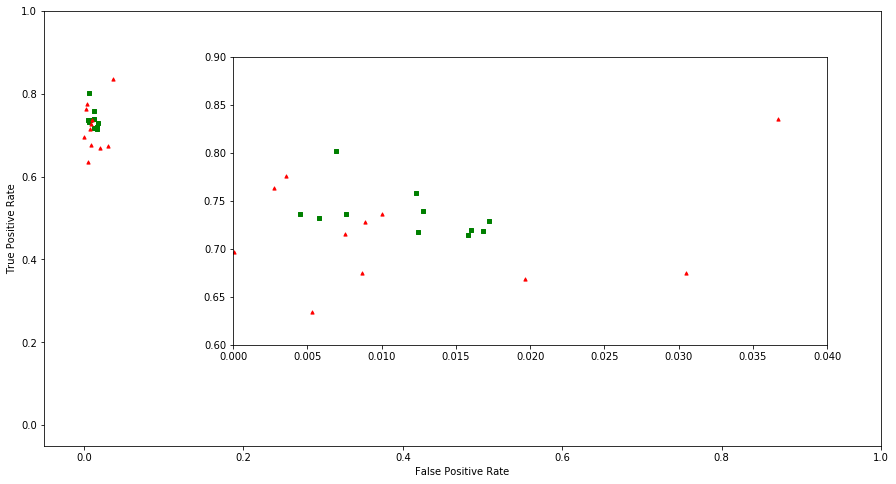
\includegraphics[width=\columnwidth]{dr_fpr_top}
	\caption{$\tpr_v$ vs. $\fpr_v$ according to $\Madups$ (green) and $\Mad$ (red).}
	\label{fig:dr_fpr_top}
\end{figure}


% To conclude the analysis of our datasets, we discuss the samples obtained from $\NSRL$~($\DNSRL$) and VirusShare.com~($\DVS$).
%We end this subsection with how the sets from \gls{nsrl} $\mathcal{D}_{NSRL}$ and VirusShare $\mathcal{D}_{VS}$ intersect our dataset $\mathcal{D}$. 
% Samples in $\DNSRL \cap \DD$ account for 4,756, while the number is 105,251 for $\DVS \cap \DD$. 

% Finally, and due to the ambiguity in the definition of malware, we also have that 426 samples are common to the three sets, \ie, are in $\DNSRL \cap \DVS \cap \DD$.

\subsection{Data Labelling}\label{sub_sec:data_labeling}
%%%%%%%%%%%%%%%%%%%%%%%%%%%%%%%%%%%%%%%%%%%%%%%
% From Data Labeling notebook
Having defined a collegiate set of vendors $\VVstar$ to classify the samples in our dataset, we can now turn our focus into labeling the reports as goodware or malware. 
To do so, we use $\CC$, together with $\NSRL$ and $\VS$, to derive three different metrics to label the reports as benign or malicious, over the set of vendors $\mathcal{V}^*$.

The first and most real metric we define is $\Mrealv$ that labels a sample $s\in\CC$ as:

\begin{itemize}
	\item $s\in\mal_\real$ if at least 5 vendors in $\VVstar$ classify $s$ positively;
	\item $s\in\good_\real$ if all vendors in $\VVstar$ classify $s$ negatively.
\end{itemize}

Since the labeling information is solely provided by $\VVstar$'s vendors, this metric's ground truth is highly dependent on their performance, which means labeling errors may be present (as we have discussed in \ref{sub_sec:data_analysis}). 
Due to this, samples that are classified positively by no more than four vendors, are discarded.

\medskip

Our second metric $\Mloosev$, restricts the previous metric $\Mrealv$ to achieve a better ground truth. We do this by including information from $\NSRL$ and VirusShare.com. 
This metric labels a sample $s\in\mathcal{C}$ as:

\begin{itemize}
	\item $s\in\mal_\loose$ if $s\in\mal_\real$ \textbf{and} it belongs to $\DVS$ and does not belong to $\DNSRL$;
	\item $s\in\good_\loose$ if $s\in\good_\real$ \textbf{and} it belongs to $\DNSRL$ and does not belong to $\DVS$.
\end{itemize}
that is
\begin{eqnarray*}
\mal_\loose&=&\left(\mal_\real\cap\DVS\right)\setminus\DNSRL\\
\good_\loose&=&\left(\good_\real\cap\DNSRL\right)\setminus\DVS
\end{eqnarray*}


By taking into account the presence in $\NSRL$, that reinforces cleanliness, and VirusShare.com, that reinforces maliciousness, this metric is more reliable, ground truth wise, at the expense of a smaller number of samples.

\medskip

Our third and final metric $\Mstrictv$, is the strictest one, labeling a sample $s\in\DD$ as:
\begin{itemize}
	\item $s\in\mal_\strict$ if all $v\in\VVstar$ classify it positively \textbf{and} $s\in\DVS\setminus\DNSRL$;
	\item $s\in\good_\strict$ if $s\in\good_\loose$.
\end{itemize}

Obviously this is the most reliable metric, in the sense that it is closely related to the samples' ground truth, leaving little room for disagreement. However, this is achieved again at the cost of a smaller number of samples.

\medskip

Taking the previously defined metrics, the task of creating labeled datasets based on them is trivial.
We apply each of the previously defined metrics, $\Mstrictv$, $\Mloosev$ and $\Mrealv$ to our classified dataset $\CC$ to obtained three new datasets, $\CC_{strict}\subseteq\CC_{loose}\subseteq\CC_{real}\subseteq\CC$.
Table \ref{tab:dataset_sizes} provides information regarding the size and number of malware and goodware in each of our datasets.

\begin{table}[!htb]
	\renewcommand{\arraystretch}{1.2} % more space between rows
	\centering
	\begin{tabular}{l|ccc}
		Dataset			& $\CC_{real}$ & $\CC_{loose}$ & $\CC_{strict}$	\\
		\hline
		Malware			& 98,582 & 45,306 & 24,658\\
		Goodware		& 56,475 & 1,989 & 1,989\\
		\hline
		Total			& 155,057 & 47,295 & 26,647\\
	\end{tabular}
	\smallskip
	\caption{Sizes for datasets $\CC_{real}$, $\CC_{loose}$ and $\CC_{strict}$.}
	\label{tab:dataset_sizes}
\end{table}
